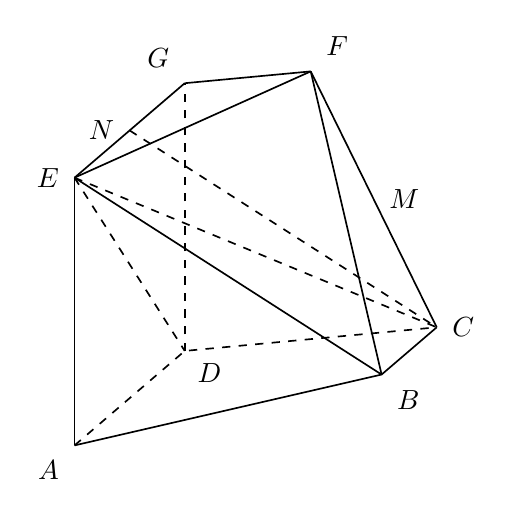
\begin{tikzpicture}[x=1cm,y=1cm,line width=.6pt]
% Space polyhedron ABCDEG F with M on FC, N on EG (positions mimic original PNG)
\coordinate (A) at (0,0);
\coordinate (B) at (3.9000000000,0.9000000000);
\coordinate (C) at (4.6,1.5);
\coordinate (D) at (1.4000000000,1.2000000000);
\coordinate (E) at (0.0000000000,3.4000000000);
\coordinate (G) at (1.4000000000,4.6000000000);
\coordinate (F) at (3.0000000000,4.7500000000);
\coordinate (M) at (3.8000000000,3.1250000000);
\coordinate (N) at (0.7000000000,4.0000000000);
% solid base + sides
\draw (A) -- (B) -- (C);
\draw (A) -- (E);
\draw (E) -- (B);
\draw (E) -- (F);
\draw (G) -- (F);
\draw (F) -- (B);
\draw (F) -- (C);
\draw (E) -- (G);
% dashed hidden + interior diagonals
\draw[dashed] (A) -- (D) -- (C);
\draw[dashed] (D) -- (G);

\draw[dashed] (E) -- (D);
\draw[dashed] (E) -- (C);
\draw[dashed] (N) -- (C);
% labels offset to avoid strokes
\node[below left=2pt] at (A) {$A$};
\node[below right=2pt] at (B) {$B$};
\node[right=2pt] at (C) {$C$};
\node[below right=1pt] at (D) {$D$};
\node[left=2pt] at (E) {$E$};
\node[above left=2pt] at (G) {$G$};
\node[above right=2pt] at (F) {$F$};
\node[right=2pt] at (M) {$M$};
\node[left=2pt] at (N) {$N$};
\end{tikzpicture}
